
\documentclass[letterpaper,11pt,titlepage,final]{report}

\usepackage{epsfig,pifont,calc,color,pstricks}
\usepackage{amsmath,latexsym,oldlfont}
\usepackage{enumerate}
\usepackage{Chicago}
\usepackage{url}

\usepackage{graphicx}
\usepackage{caption}


%\def\ImPath{/home/ampuero/WAVES/SEM2DPACK_2.x/doc/FIGURES}
%\def\ImPath{../FIGURES}
%\def\Version{2.3.8}
\def\MonthYear{March 2017}

%%%%%%%%%%%%%%%%%%%%%%%%%%%%
%% A4 wide
%%%%%%%%%%%%%%%%%%%%%%%%%%%%
 
\usepackage{a4wide}
%\textwidth 16.7cm
%\textheight 24.6cm
%\oddsidemargin -4.5mm
%\evensidemargin -4.5mm
%\topmargin -11.5mm
 
%%%%%%%%%%%%%%%%%%%%%%%%%%%%
%% US letter
%%%%%%%%%%%%%%%%%%%%%%%%%%%%
 
%\textwidth 17cm
%\textheight 23.8cm
%\oddsidemargin -4.5mm
%\evensidemargin -4.5mm
%\topmargin -22.5mm
 
%%%%%%%%%%%%%%%%%%%%%%%%%%%%

%\usepackage{fancyheadings}
\usepackage{fancyhdr}
\pagestyle{fancyplain}
\renewcommand{\chaptermark}[1]{\markboth{#1}{#1}}
\renewcommand{\sectionmark}[1]{\markright{\thesection\ #1}}
\lhead[\fancyplain{}{\bfseries\thepage}]{\fancyplain{}{\bfseries\rightmark}}
\rhead[\fancyplain{}{\bfseries\leftmark}]{\fancyplain{}{\bfseries\thepage}}
\cfoot{}
\renewcommand{\labelitemii}{{\LARGE\bf .}}

% pour voir la bounding box postscript
%\newcommand{\voirbbox}[1]{{\fboxsep 0pt \fbox{#1}}}

% pour ne pas la voir
\newcommand{\voirbbox}[1]{{{#1}}}

%
% define new items (necessite package pifont)
%

\font\pzdr=pzdr at 12pt

\newenvironment{fancyitemize}[1]
   {\begin{itemize}
    \renewcommand{\labelitemi}{{\pzdr #1}}
    \renewcommand{\labelitemii}{{\pzdr #1}}
    \renewcommand{\labelitemiii}{{\pzdr #1}}
   }
   {\end{itemize}}

%
% define new enumerate (necessite package pifont et calc)
%

\newcounter{local}

\newenvironment{enumerateW}
   {
     \begin{enumerate}
     \renewcommand{\labelenumi}{\setcounter{local}{191+\value{enumi}}\ding{\value{local}}}
     \renewcommand{\labelenumii}{\setcounter{local}{191+\value{enumii}}\ding{\value{local}}}
     \renewcommand{\labelenumiii}{\setcounter{local}{191+\value{enumiii}}\ding{\value{local}}}
   }
   {\end{enumerate}}

\newenvironment{enumerateB}
   {
     \begin{enumerate}
     \renewcommand{\labelenumi}{\setcounter{local}{201+\value{enumi}}\ding{\value{local}}}
     \renewcommand{\labelenumii}{\setcounter{local}{201+\value{enumii}}\ding{\value{local}}}
     \renewcommand{\labelenumiii}{\setcounter{local}{201+\value{enumiii}}\ding{\value{local}}}
   }
   {\end{enumerate}}

\newcommand{\relief}[1]{{\it\bfseries #1}}

%%%%%%%%%%%%%%%%%%%%%%%%%%%%%%%%%%%%%%%%%%%%%%%%%%%%%%%%%%%%%%%%%%
% FIGURES:

\newcommand{\Img}[2]{
\begin{minipage}{#2\linewidth}
\centerline{ \epsfig{file=\ImPath/#1,width=\linewidth}}
\end{minipage}
}

\newcommand{\ImgC}[2]{
\centerline{ \epsfig{file=\ImPath/#1,width=#2\linewidth} }
}

\newcommand{\ImgL}[2]{
\begin{minipage}{#2\linewidth}
\centerline{ \epsfig{file=\ImPath/#1,width=\linewidth,angle=-90}}
\end{minipage}
}

\newcommand{\ImgCL}[2]{
\centerline{ \epsfig{file=\ImPath/#1,width=#2\linewidth,angle=-90} }
}

%%%%%%%%%%%%%%%%%%%%%%%%%%%%%%%%%%%%%%%%%%%%%%%%%%%%%%%%%%%%%%%%%%%%%
% EQUATIONS:
\newcommand{\eq}{\begin{equation}}
\newcommand{\en}{\end{equation}}
\newcommand{\eqa}{\begin{eqnarray}}
\newcommand{\ena}{\end{eqnarray}}

%%%%%%%%%%%%%%%%%%%%%%% REFERENCES %%%%%%%%%%%%%%%%%%%%%%%%%%%%%%%%%%%
\newcommand{\Eqref}[1]{Equation~\ref{Eq:#1}}
\newcommand{\figref}[1]{Figure~\ref{Fig:#1}}
\newcommand{\secref}[1]{Section~\ref{Sec:#1}}
\newcommand{\charef}[1]{Chapter~\ref{Cha:#1}}
\newcommand{\appref}[1]{Appendix~\ref{App:#1}}
\newcommand{\tabref}[1]{Table~\ref{Tab:#1}}

%%%%%%%%%%%%%%%%%%%%%%%%%%%%%%%%%%%%%%%%%%%%%%%%%%%%%%%%%%%%%%%%%%%%%
% SHORTER ITEMIZE
\newenvironment{sitemize}
{\begin{list}{--}%
  {\setlength{\topsep}{0pt}%
   \setlength{\itemsep}{0pt}%
   \setlength{\leftmargin}{2em} }}
{\end{list}}

\newenvironment{senumerate}
{\begin{enumerate}
  \setlength{\topsep}{0pt}
  \setlength{\itemsep}{0pt}
  \setlength{\parskip}{0pt}
  \setlength{\parsep}{0pt}}
{\end{enumerate}
}

%%%%%%%%%%%%%%%%%%%%%%%%%%%%%%%%%%%%%%%%%%%%%%%%%%%%%%%%%%%%%%%%%%%%%

%\includeonly{chap1}

%
% Start the Report
%
\begin{document}

\parindent 0pt
\parskip 10pt

%%%%%%% TITLE PAGE %%%%%%%%%%%%%%%%%%%%%%%%%%%%%%%

\thispagestyle{empty}
\vspace*{\fill}
\begin{center}

%\pspicture(15.5,0)
%\psline[linestyle=solid,linecolor=red,linewidth=2pt](-0.1,0)(15.6,0)
%\endpspicture

\vspace*{1mm}
{\Huge\bf{ 1D-3C SEM}}\\[5mm]
{\Large A Spectral Element Method tool for 1D wave propagation }\\
{\Large with three components (3C) in linear and nonlinear media}\\[2mm] 
{\Large \bf{User's Guide}}

%\pspicture(15.5,0)
%\psline[linestyle=solid,linecolor=red,linewidth=1.5pt](-0.1,0.2)(15.6,0.2)
%\endpspicture

\newfont{\fdunB}{cmdunh10 scaled \magstep2}
\vspace*{3cm}
\fdunB
%Version \Version \\[3mm]
\MonthYear \\[3cm]
Elif ORAL\\[2mm]
{\small

E-mail: 1d3csem@gmail.com \\
}
\end{center}
\vfill
%\newpage
\thispagestyle{empty}
\hspace*{0pt}
\newpage
\thispagestyle{empty}
\vspace*{\fill}
%\centerline{ \copyright\ 2003-2012 Jean-Paul Ampuero}

%%%%%%% TABLE OF CONTENTS %%%%%%%%%%%%%%%%%%%%%%%%%%%%%%%%%%%%%%%%%%%%%%

\newpage
{\parskip 0pt
  \tableofcontents
}
\newpage

%%%%%%% BODY %%%%%%%%%%%%%%%%%%%%%%%%%%%%%%%%%%%%%%%%%%%%%%%%%%%%%
\chapter{Introduction}


The 1D-3C SEM code is a numerical tool for spectral element modeling (SEM) of one-dimensional (1D) seismic wave propagation with three components (3C) in linear and nonlinear media. It is an extended version of the 1D SEM code supplied by the PhD work of Elise Delavaud \cite{Delavaud2007}. The additional contributions have been made by Elif Oral during her PhD thesis \cite{Oral2016}. \\

The 1D-3C SEM code offers many choices for the soil rheology in propagation medium and bottom boundary conditions. As soil constitutive model (soil rheology), it is possible to model elasticity, viscoelasticity, elastoplasticity and visco-elastoplasticity. For boundary conditions, 1D-3C SEM allows for defining rigid condition, absorbing layer condition with Perfectly Marched Layers (PML), borehole condition and free surface condition. \\

For viscoelastic attenuation in propagation medium, \cite{LiuArchuleta2006} model has been implemented in the code, whereas soil nonlinearity is based on MPII model of \cite{Iwan1967}. For nonlinearity, the code offers pressure-dependent and pressure-independent modeling possibilities. For pressure-independent models, it is possible to define soil nonlinearity with given experimental data or hyperbolic curve of  \cite{HardinDrnevich1972}. Furthermore, in pressure-dependent models, effective and total stress analyses could be performed. The excess pore pressure development in effective stress analysis is modeled in 1D-3C SEM code following the front saturation model of \cite{Iaietal1990}. For more details on theory of these models, the user is invited to refer to \cite{Oral2016}. \\


The 1D-3C SEM code is a completely free (open) source and it is provided with several example files and Python-based scripts to be used for pre- and post-treatments.  In the following, first, the compilation of the code is detailed. Second, the employment of different models into the code is explained by means of various examples. Lastly, the use of available python scripts are given. \\

\chapter{Compilation}

The compilation of 1D-3C SEM code is tested for gfortran and ifort compilers. A faster computation is provided by optimization options with the compiler flags. In order to compile the code, the user should execute ‘make’ command first  in ‘SRC/Modules’ folder, where the ‘Makefile’ is available for modules. The same execution should be applied in ‘SRC’ folder, where another ‘Makefile’ is available for main fortran files. This procedure is written in compile.sh file. It is also possible to use directly this bash file for compilation.  \\

For both compilers (gfortran and ifort), necessary flags are provided in Makefile.  For users who prefer gfortran compiler, necessary flags are as follows:\\

OPT  = -O2 -finline-functions -funswitch-loops -fpredictive-commoning \
                  -fpredictive-commoning  -fgcse-after-reload -ftree-slp-vectorize  \
                  -ftree-loop-distribute-patterns -fvect-cost-model -fipa-cp-clone  \
                  -fno-math-errno -funsafe-math-optimizations  \
                  -fno-rounding-math -fno-signaling-nans -fcx-limited-range  \
                  -g3 -fbacktrace  -fdefault-double-8 -fdefault-real-8 -fdefault-integer-8

This option is equivalent to the Ofast and avoids possible computational errors. For the use of ifort compiler, following command is suggested:\\

OPT= -O3 -ip -ipo -unroll

Advanced users who intend to change the content of source files are suggested to specify dependencies in Makefile.depend files in ‘Modules’ directory.\\

Once the compilation is completed, the code creates an executable in upper directory which is named ‘SEM1D3C’. Then, the user could perform simulations in her working directory with this executable.\\

\chapter{Examples}

\section{Introduction}
The 1D-3C SEM code is served to use with several examples which had been used in analyses of \cite{Oral2016}. First, for an elastic medium assumption, the realistic model of Volvi (Greece) is given. Second, the same model of Volvi is used with viscoelastic soil constitutive model. Afterwards, nonlinear examples are shown for different cases. One of the nonlinear cases is the pressure-independent P1 model. The soil nonlinearity in this model is considered by elastoplasticity where 50 Iwan mechanisms are defined. Another nonlinear case is the pressure-dependent model of Wildlife Refuge Liquefaction Array (WRLA) which is provided with total and effective stress analyses. Lastly, effective stress analysis of Kushiro port (KP) site model which is initially anisotropically consolidated is provided. These examples are detailed by input and output files below.\\


\section{Elasticity model}

For elasticity, Volvi model example is given. It can be found in EXAMPLES\slash VOLVI\slash ELASTIC directory. The model is composed of eight soil layers. In the table below, main properties of the model are shown, where $\rho$ is soil density, $V_{s}$ and $V_{p}$ are shear and pressure wave velocities, $Q_{s}$ and $Q_{p}$ are quality factors for shear and pressure waves, respectively. For elasticity, $Q_{s}$ and $Q_{p}$ values are ignored. \\


\vspace{1cm}
% Table : Volvi soil ppts
\captionof{table}{Soil properties at the Volvi model.}
\label{TABvolvi}
\begin{center}
\begin{tabular}{|c|c|c|c|c|c|c|c|} \hline                                
Layer  & Thickness $[m]$ & $V_{s} [m/s] $ &  $V_{p} [m/s] $   & $\rho [kg/m^{3}]$ & $Q_{s}$& $Q_{p}$  \\ \hline \hline 
1     & 7    	& 130 	& 1500  & 2050   &  15 	  & 75  \\ \hline    
2     & 13     	& 200   & 1500	& 2150   &  20    & 75  \\ \hline    
3     & 34    	& 300   & 1650	& 2075   &  30    & 83  \\ \hline    
4     & 23.5    & 450   & 2050	& 2100   &  40    & 103 \\ \hline    
5     & 50    	& 600   & 2450	& 2155   &  60    & 123	\\ \hline    
6     & 59    	& 700   & 2550	& 2200   &  70    & 140	 \\ \hline    
7     & 10    	& 1250  & 3500	& 2500   &  100   & 200  \\ \hline    
Bedrock& 103.5  & 2600  & 4500	& 2600   &  50000 & 50000 \\ \hline    
\end{tabular}
\end{center}

In this example, upper boundary is defined as free surface and at bottom of the model, PML (Perfectly Matched Layers) is used. It should be noted that 1D-3C SEM code assumes use of a single element for PML. For further changes, the user could make modifications  in the code by ‘sigeps.f90’ file. \\


The first file that the user should provide is ‘input.spec’, which is shown in the following figure of Volvi model. \\

% FIGURE : INPUT.SPEC
\begin{center}
\leavevmode
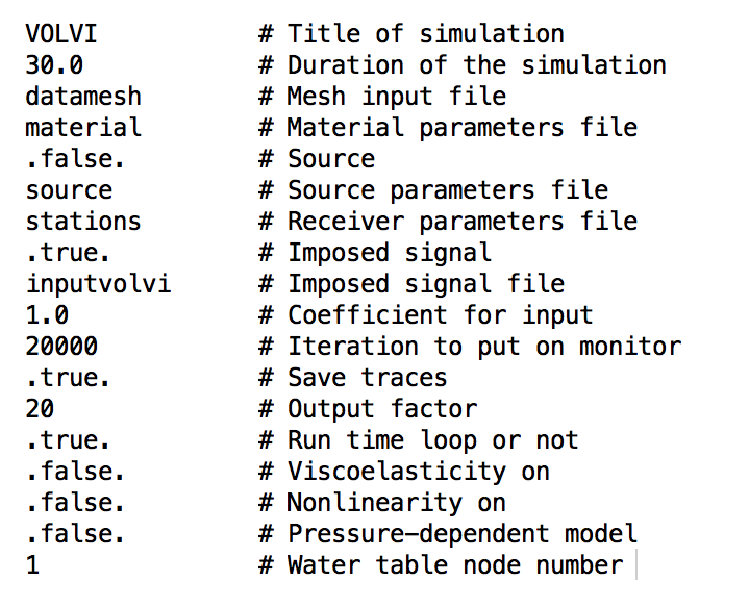
\includegraphics [scale=0.75] {figures/inputspec.eps} 
\label{inputspec} 
\captionof{figure}{Input file input.spec for elastic Volvi model.}
\vspace{1cm}
\end{center}


The file is self-explanatory. Title of simulation and total duration of simulation should be specified. Then, the mesh file name from which the necessary data about element and domain characteristics are to be read is needed. In pre-treatment section of this manual, an example for creating a mesh file is given. \\

For material properties, the code requires a file which respects the following format. The user should define total number of domains. Then , for each domain, P and S velocity values, density, PML condition (True \slash False), time step of simulation, GLL number, viscoelasticity quality factors for P and S waves, reference frequency and nonlinear soil type should be written. Although same time step is used all over the model, the format requires entering this data for each domain. For elastic models, even though it is not necessary viscoelastic or nonlinear parameters in computations, the user should follow the specified format for every model. For PML domain, n and A coefficients are necessary.  If no PML is used, the PML data section should be left commented. Lastly, for pressure-dependent models, for each domain, the user must define whether excess pore pressure development is expected (T) or not (F) and pressure-dependent soil type. In other models such as this elastic example, this part will be ignored. However, the user should create the material file in this format. \\

% FIGURE : MATERIAL
\begin{center}
\leavevmode
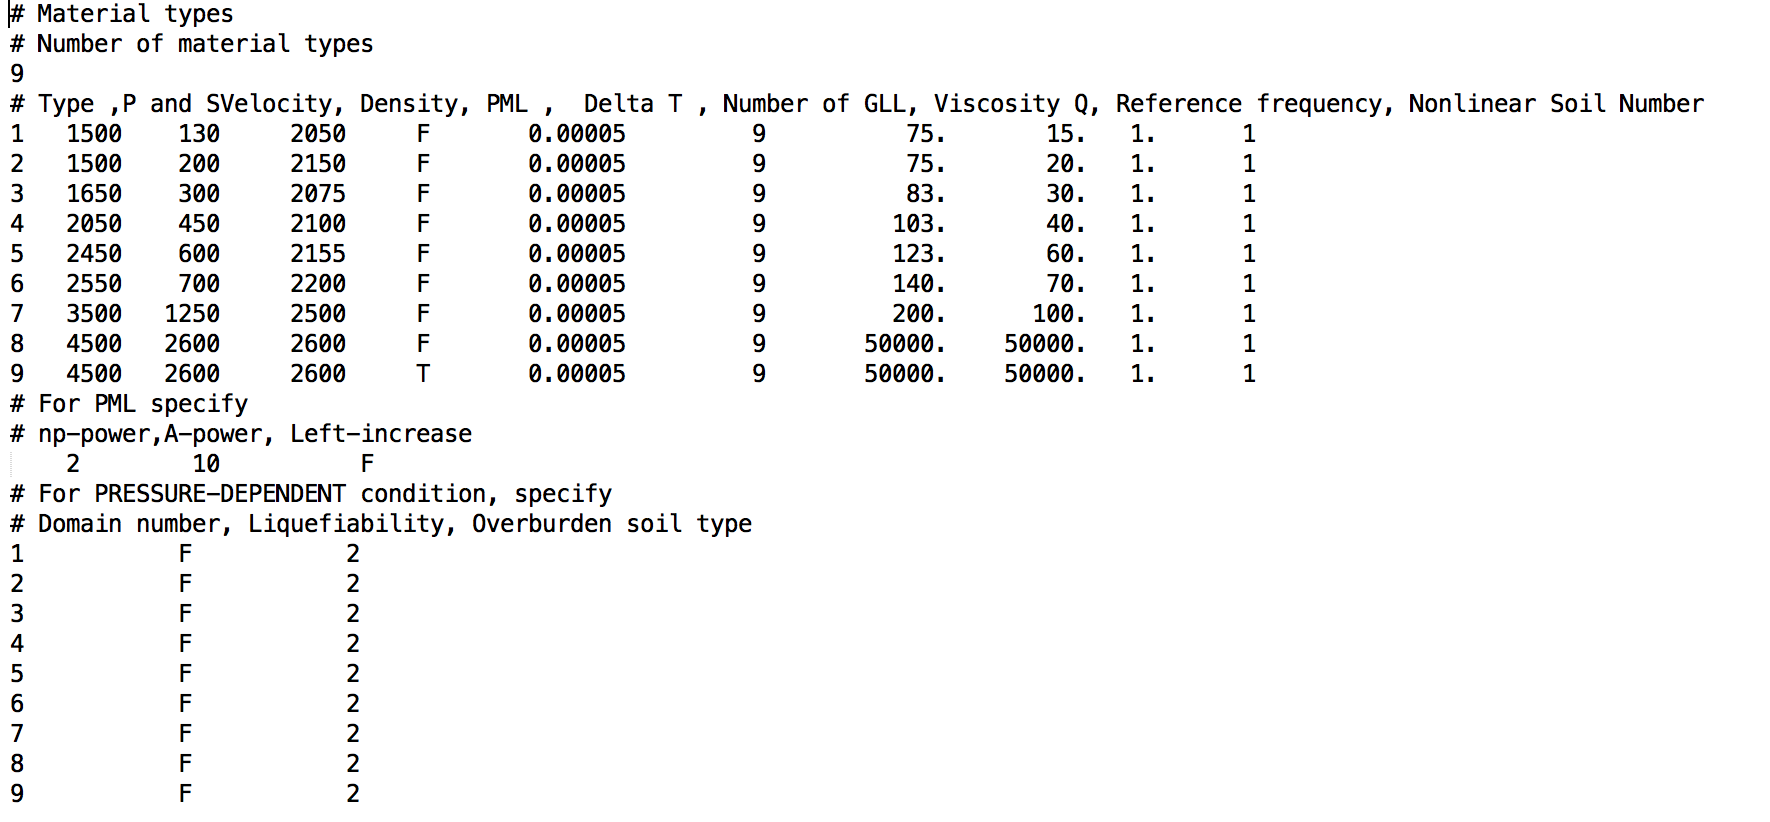
\includegraphics [scale=0.6] {figures/material.eps} 
\captionof{figure}{Material file for elastic Volvi model.}
\label{mat} 
\vspace{1cm}
\end{center}


When we come back to input file, the following input data concerns sources. For cases where point source is defined as input motion, the user should set source option should be defined as ‘.True.’ and specify file name in which source type and properties are given . Such a source file should contain: \\

\begin{enumerate}

\item Coordinate
\item Source kind (1 for impulse; 2 for explosion)
\item Source function (1 for Gaussian; 2 for Ricker)
\item Pulse width (Only if Gaussian type of function is given)
\item Delay time  (Only if Ricker type of function is given)
\item Cut-off frequency (Only if Ricker type of function is given)

\end{enumerate}


For cases where the input motion is defined by an incident wave field, the code requires a file in which time step and corresponding velocity of incident wave are included. It should be noted that time step of the input motion should not be smaller than time step of simulation. For such cases, the user should write ‘.True.’ for imposed signal and file name for imposed signal file. It is also possible to define a coefficient for the given velocity field. \\

The receiver coordinates should be included in a file with total number of stations. An example is given below: \\

% FIGURE : STATIONS
\begin{center}
\leavevmode
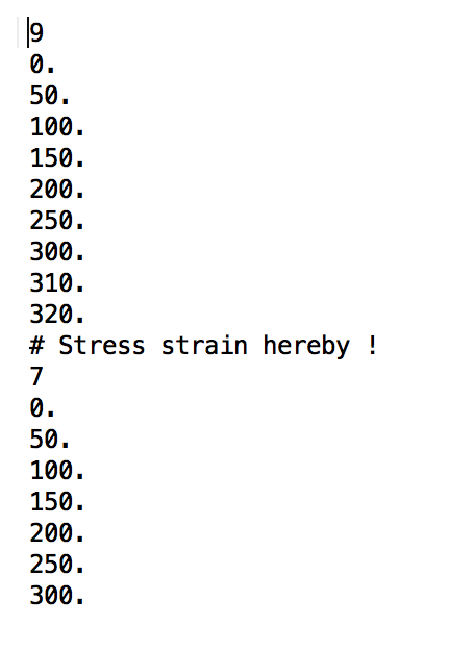
\includegraphics [scale=0.75] {figures/stations.eps} 
\captionof{figure}{Station (receiver) file for elastic Volvi model.}
\label{stat} 
\vspace{1cm}
\end{center}

In receiver file (‘stations’ in this example), first, the receivers where acceleration, velocity time histories are desired as output are defined. In the second part of the file, different depths could be defined for saving nonlinearity and pore pressure model parameters. More details about output files are given in last chapter of this manual (See Chapter \ref{sec:prepost}). \\

When the code is executed, some information are written out in terminal as below : \\

% FIGURE : TERMINAL
\begin{center}
\leavevmode
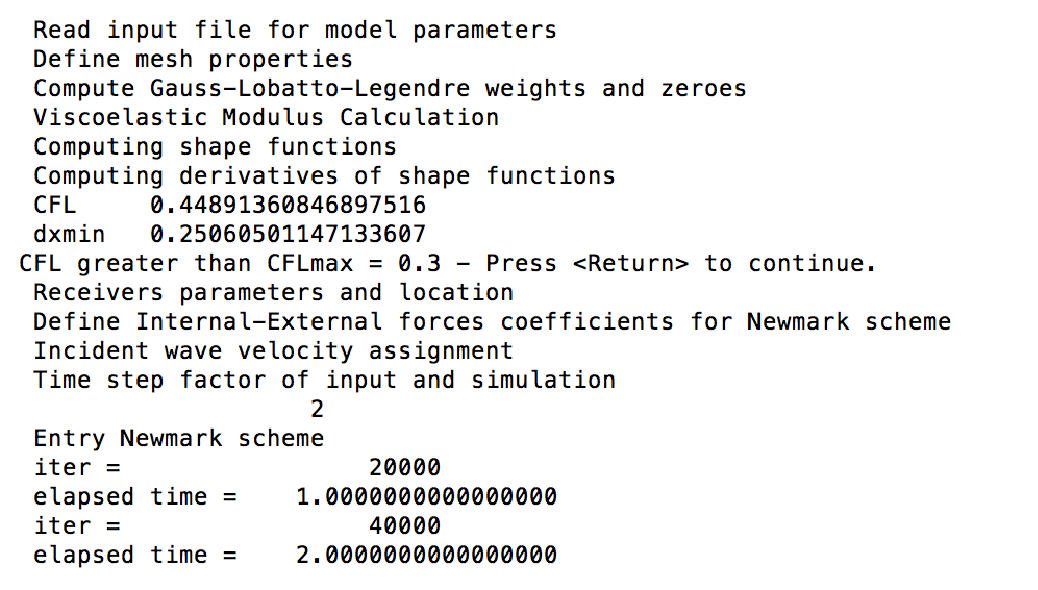
\includegraphics [scale=0.75]{figures/terminal.eps} 
\captionof{figure}{Output data in terminal for 2 seconds of simulation in elastic Volvi model.}
\label{ter} 
\vspace{1cm}
\end{center}


In order to control the time interval of output information concerning elapsed time, the user could change the iteration number in input.spec file by ‘iteration to put on monitor’. For the simulations where the user does not want to perform time iterations but verifies the execution of the code (useful for further modifications by advanced users), ‘Run time loop’ could be chosen as ‘.False.’. Also, if the user does not want to save output files, ‘Save traces’ should be chosen as False. Otherwise, at the end of simulation, the code provides output files at given receiver coordinates. \\

Lastly, the soil constitutive models should be defined. For elasticity, the user should set ‘Viscoelasticity on’, ‘Nonlinearity on’ and ‘Pressure-dependent model’ False. The other cases will be detailed in following sections. For elasticity, ‘Water table node’ is not taken into consideration in computations. \\



\section{Viscoelasticity model}

Viscoelasticity example could be found in EXAMPLES\slash VOLVI\slash VISCOELASTIC directory.  For viscoelasticity, compared to elasticity, the changes apply to input.spec and material files. In input.spec files, differently than elasticity, ‘Viscoelasticity on’ should be set to ‘True’. In material file, quality factors for P and S waves with reference frequency (which will be no longer ignored by the code) should be provided for each domain. 


\section{Nonlinearity model}

\subsection{Pressure-independent nonlinearity}

For pressure-independent nonlinear model, an example is given in EXAMPLES\slash P1 directory.  The model is composed of a single layer with following properties: \\

\vspace{1 cm}
% Table : WL soil ppts
\captionof{table}{Soil properties at P1 model (PRENOLIN).}
\label{tabP1}
\begin{center}
\begin{tabular}{|c|c|c|c|c|c|c|} \hline                                
Layer & Thickness $[m]$ & $V_{s} [m/s] $ &$V_{p} [m/s] $ & $\rho [kg/m^{3}]$ & $Q_{s}$ & $Q_{p}$ \\ \hline \hline 
1     &  20   		& 300  		& 700 		&  2000 	     & 30  & 70  \\ \hline    
\end{tabular}
\end{center}


In such a case, the user should define, first, in input.spec file, ‘Nonlinearity on’ as True, so that the model follows elastoplasticity. If viscous attenuation is also demanded, then ‘Viscoelasticity on’ must be set to True as well, such that the model is visco-elastoplastic. \\

Also, for nonlinearity, another file which should be named ‘GoverGmax.dat’ is required, differently than elastic and viscoelastic cases. The format of the file is shown below: \\

% FIGURE : GoverGmax.dat
\begin{center}
\leavevmode
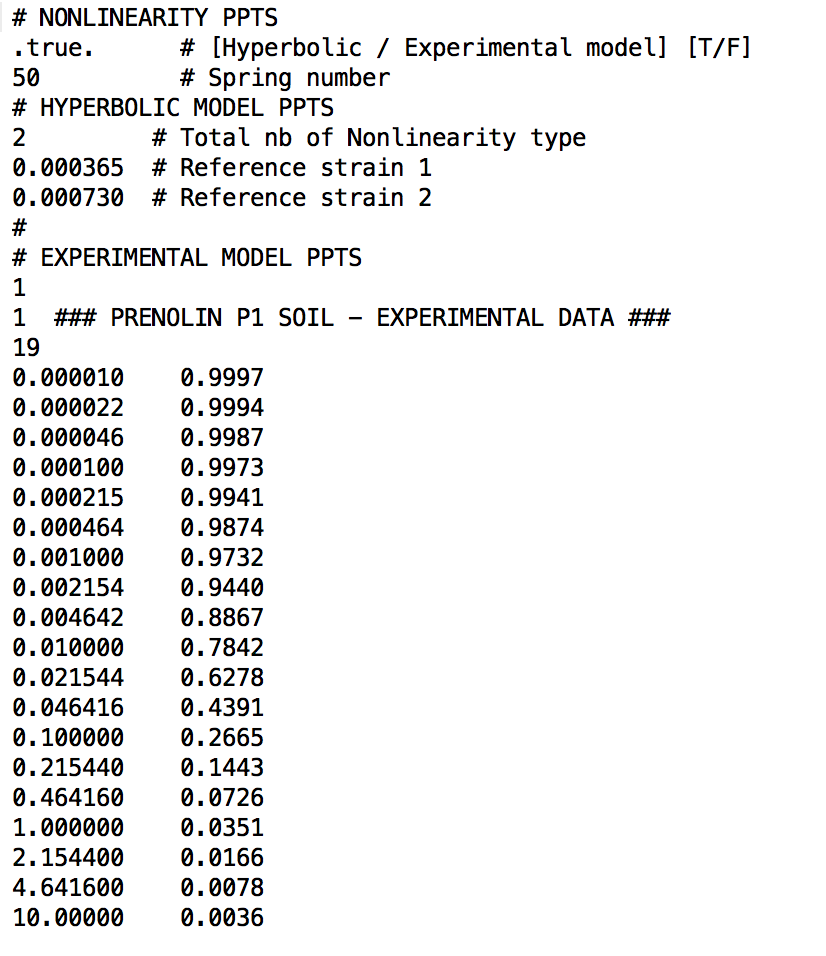
\includegraphics [scale=0.75] {figures/GoverGmaxdat.eps} 
\captionof{figure}{GoverGmax.dat file for P1 example.}
\label{GG} 
\vspace{1cm}
\end{center}

In this latter, the choice of hyperbolic or experimental model in order to construct the backbone curve should be made. For hyperbolic models, the Equation \ref{eqHD} is used so that the user must define a reference strain. \\


% Equation - Hardin and Drnevich 1972
\begin{equation}
\label{eqHD}
\frac{G}{G_{0}} = \frac{1}{1+ \gamma / \gamma_{ref}} 
\end{equation}


In this example, two different values are available. In ‘material’ file, the nonlinear soil type should be written according to the reference strain data in this file, for hyperbolic models. Otherwise, the user has the possibility of defining an experimental curve by giving strain (in percentage) and corresponding shear modulus ratio. Again, the soil type must match with the defined nonlinear soil type in ‘material’ file for each domain. Lastly, in the same file, the total number of Iwan springs is obligatorily given for all nonlinear cases. In this example, it is set to 50. \\


\subsection{Pressure-dependent nonlinearity}

For pressure-dependent model, Wildlife Refuge Liquefaction Array site model is given.  The model is composed of four layers of which only the third layer is liquefiable. In other words, only in the third layer, excess pore pressure development is expected to be developed. \\



% Table : WL soil ppts
\captionof{table}{Soil properties at Wildlife Refuge Liquefaction Array after \protect\cite{Bonilla2005} }
\begin{center}
\begin{tabular}{|c|c|c|c|c|c|c|c|} \hline                                
Layer & Description  & Thickness $[m]$ & $V_{s} [m/s] $ &$V_{p} [m/s] $ & $\rho [kg/m^{3}]$ & $\phi_{f} [degree]$ & $K_{0}$ \\ \hline \hline 
1     & Silt    		& 1.5   & 99  & 249 &  1600 & 28  & 1.0  \\ \hline    
2     & Silt    		& 1.0   & 99  & 281 &  1928 & 28  & 1.0  \\ \hline
3     & Silty sand 	& 4.3   & 116 & 1019&  2000 & 32  & 1.0  \\ \hline
4     & Silty sand 	& 0.7   & 116 & 1591&  2000 & 32  & 1.0  \\ \hline
\end{tabular}
\label{TAB:WRLA1}
\end{center}



For this site, the models of effective and total stress analyses are provided. First, necessary modifications for total stress analysis are detailed. Then, further changes to be made for effective stress analysis are explained. \\

\paragraph{Total stress analysis}

For total stress analysis, in other words, for pressure-dependent nonlinear models where no excess pore pressure develops, the first change applies to ‘input.spec’ file. The user should define ‘Nonlinearity on’ and ‘Pressure-dependent model’ as True. The water level should be defined by the corresponding node number in mesh file. This means that if water level is present in the model, it must correspond to an elementary boundary in the model.  \\

In addition, differently than previous cases, in pressure-dependent model, another file ‘pressparam.dat’ is required. The format of the file is given below.  In this file, m1 (slope of the soil failure line), cohesion and coefficient of Earth at rest are compulsory for total stress analysis. Other parameters are to be neglected in total stress analysis computations. \\

%% FIGURE : pressparam.dat
\begin{center}
\leavevmode
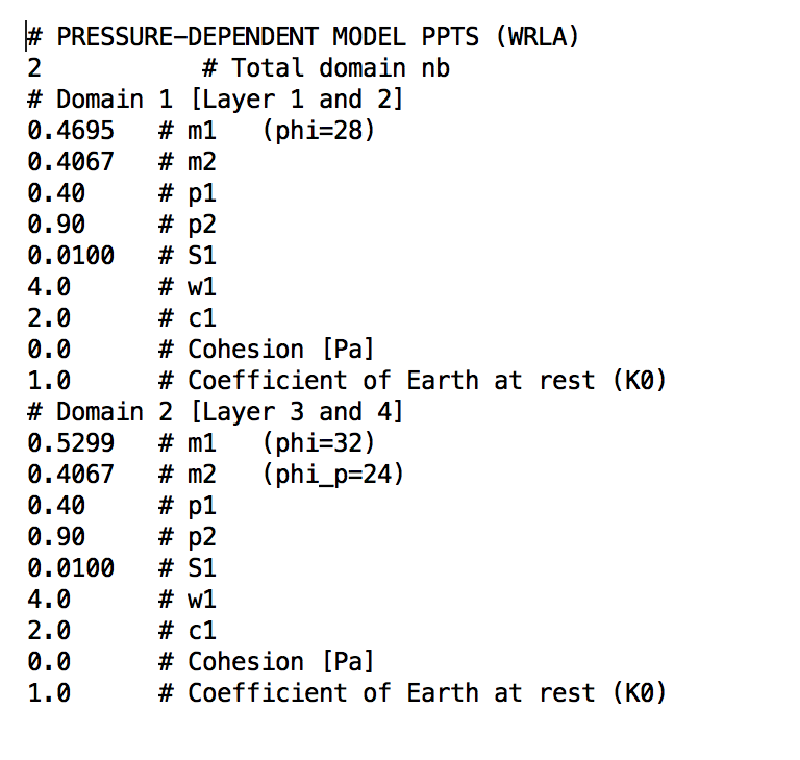
\includegraphics [scale=0.75] {figures/pressparamdat.eps} 
\captionof{figure}{pressparam.dat file for P1 example.}
\label{press} 
\vspace{1cm}
\end{center}


Accordingly, in the last part of the material file, the overburden soil type should match the soil number in ‘pressparam.dat’ soil types. For total stress analysis, each domain is non-liquefiable such that liquefiability is specified as False. \\


\paragraph{Effective stress analysis}

Effective stress analysis for WRLA model can be found in EXAMPLES\slash WRLA\slash EFFECTIVE \textunderscore STRESS\textunderscore ANALYSIS directory. In WRLA model, the third layer is assumed to be liquefiable. This property is defined in the liquefiability part of the material file. For this example, the third layer liquefiability is True while other layers are False, as seen in Figure \ref{matwrla}. 


% FIGURE : MATERIAL WRLA
\begin{center}
\leavevmode
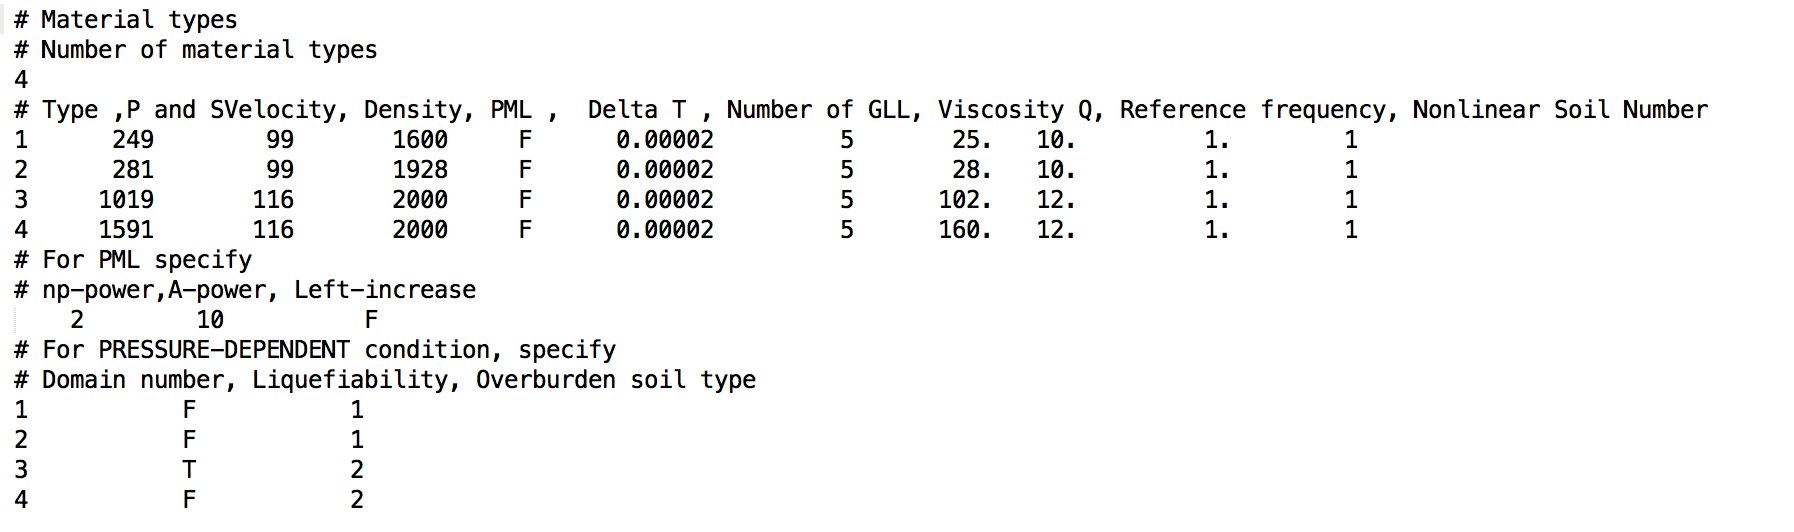
\includegraphics[scale=0.6]{figures/mat2.eps} 
\captionof{figure}{Material file for WRLA effective stress analysis model.}
\label{matwrla} 
\vspace{1cm}
\end{center}

Compared to total stress analysis, another change is made in pressparam.dat file. The model properties necessary for pore pressure excess computation such as $m_{2}$, $p_{1}$, $p_{2}$, $S_{1}$ and $w_{1}$ (front saturation model parameters) are required for the liquefiable layer. In this example, the third layer corresponds to the  overburden soil type 2. Thus, in pressparam.dat file, the code looks for the front saturation model parameters for that soil type. 

\paragraph{Effective stress analysis - II}

Another example is given for effective stress analysis in Kushiro Port model (KP), which is initially consolidated in anisotropic conditions. The KP model properties are given in Table \ref{KUSH2}. \\


\vspace{1cm}
% Table : KP soil ppts
\captionof{table}{Soil properties at Kushiro Port vertical array after \protect\cite{Iai1995}. $V_{p}$ values are calculated by assumption of Poisson ratio equal to $0.48$. }
\begin{center}
\begin{tabular}{|c|c|c|c|c|c|c|c|} \hline                                
Layer & Description  & Thickness $[m]$ & $V_{s} [m/s] $ &$V_{p} [m/s] $ & $\rho [kg/m^{3}]$ & $\phi_{f} [degree]$ & $K_{0}$ \\ \hline \hline 
1     & Fill soil    	& 2.0    	& 249  & 1270 	&  1540 & 40 & 0.5  \\ \hline    
2     & Sand    	& 7.0    	& 249  & 1270	&  1720 & 40 & 0.5  \\ \hline
3     & Sand	 	& 14.0   	& 326  & 1662 	&  1980 & 48 & 0.5  \\ \hline
4     & Silt 		& 9.0    	& 265  & 1351 	&  1730 & 37 & 0.5  \\ \hline
5     & Silt 		& 4.0    	& 341  & 1739 	&  1760 & 44 & 0.5  \\ \hline
6     & Silt 		& 8.0    	& 286  & 1458 	&  1700 & 44 & 0.5  \\ \hline
7     & Silt 		& 8.0    	& 302  & 1540 	&  2000 & 45 & 0.5  \\ \hline
8     & Silt 		& 25.0   	& 341  & 1739 	&  1730 & 44 & 0.5  \\ \hline
\end{tabular}
\label{KUSH2}
\end{center}


Since the model has a coefficient of Earth at rest equal to 0.5 for each layer, this property is defined in ‘pressparam.dat’ file with K0 parameter. \\

\chapter{Prior and posterior analyses}

\section{Pre-treatment}

1D-3C SEM codes provides PRE and POST folders for simple prior and posterior analyses to simulations. First, in PRE directory, a Python script ‘create \textunderscore mesh.py’  is provided for mesh file creation which is required for the code to define the coordinates of element nodes and boundary conditions. \\

The script is self-explanatory and interactive. First, the user is asked to specify the name of the mesh file to be created and its explanation. Then, total element number, total domain number and upper boundary condition should be defined. Afterwards, the script needs the set of element sizes to be used. In Figure \ref{cremesh}, an example for a model of 20 meters depth which is composed of two elements is shown. Once element sizes are defined, for each domain of the model, the scripts asks total number of element for each element size. To finish, bottom boundary condition is necessary. \\



%% FIGURE : create_mesh.py
\begin{center}
\leavevmode
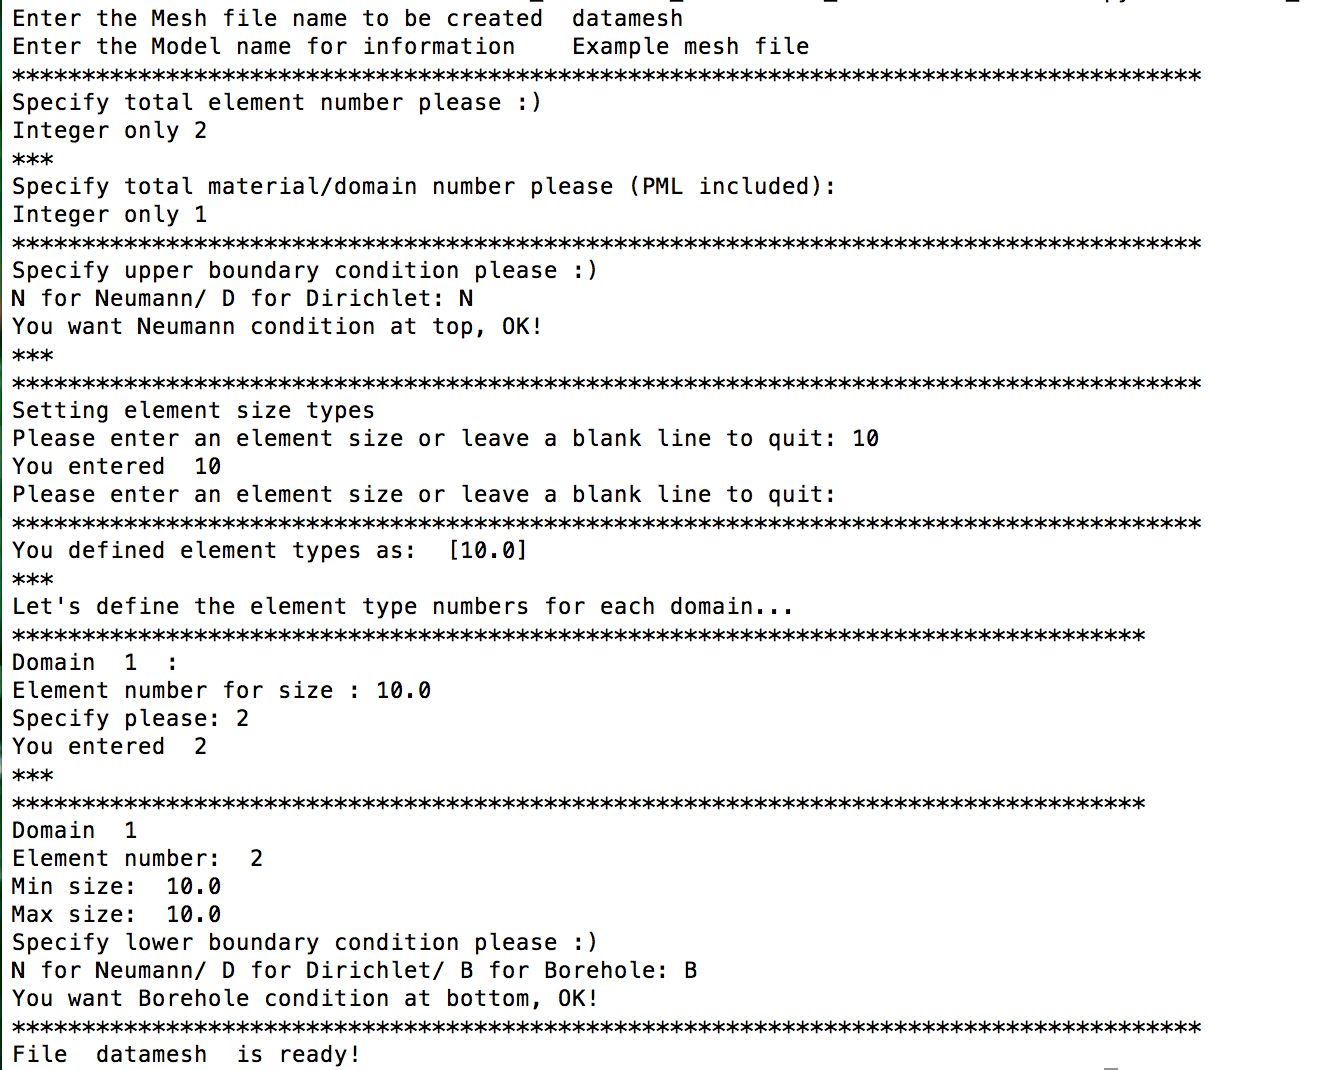
\includegraphics[scale=0.65]{figures/createmeshpy.eps} 
\captionof{figure}{create \textunderscore mesh.py file for 1D mesh file creation.}
\label{cremesh} 
\vspace{1cm}
\end{center}



\section{Post-treatment}

\label{sec:prepost}

Once the simulation terminates, the code sorts a number of output files. For all rheological models (elastic, viscoelastic, nonlinear cases), acceleration, velocity time histories in three directions of the first series of receivers are saved. Also, stress and strain parameters for the second series of receivers are written out in files. \\ 

For pressure-independent nonlinear models, such as P1 example, additionally a file with backbone curve strain and stress parameters is furnished. Depending on curve type (hyperbolic or experimental), the file name is named SOILHYPER or SOILEXP.  \\


For pressure-dependent models,  two additional files are provided. ‘PressSoilParams00X.dat’ file (where X refers to receiver number) includes shear modulus, Young modulus, bulk modulus, Poisson ratio, initial shear modulus after normalization and current maximum shear modulus, for each time step. In ‘PressEffectiveParams00X.dat’, current values of principal deviatoric stress, $W_{s}$, $W_{n}$, $S_{0}$ and $S$ parameters of the front saturation model, pore pressure excess and reference strain are given.   \\

As posterior analyses, in POST directory, other Python-based scripts are provided to users of 1D-3C SEM code. The first file is called ‘accel \textunderscore sigeps.py’ which plots acceleration time histories and stress-strain curves for given files. Resultant figure for P1 model is shown in \ref{plot}.


%% FIGURE : plot.png
\begin{center}
\leavevmode
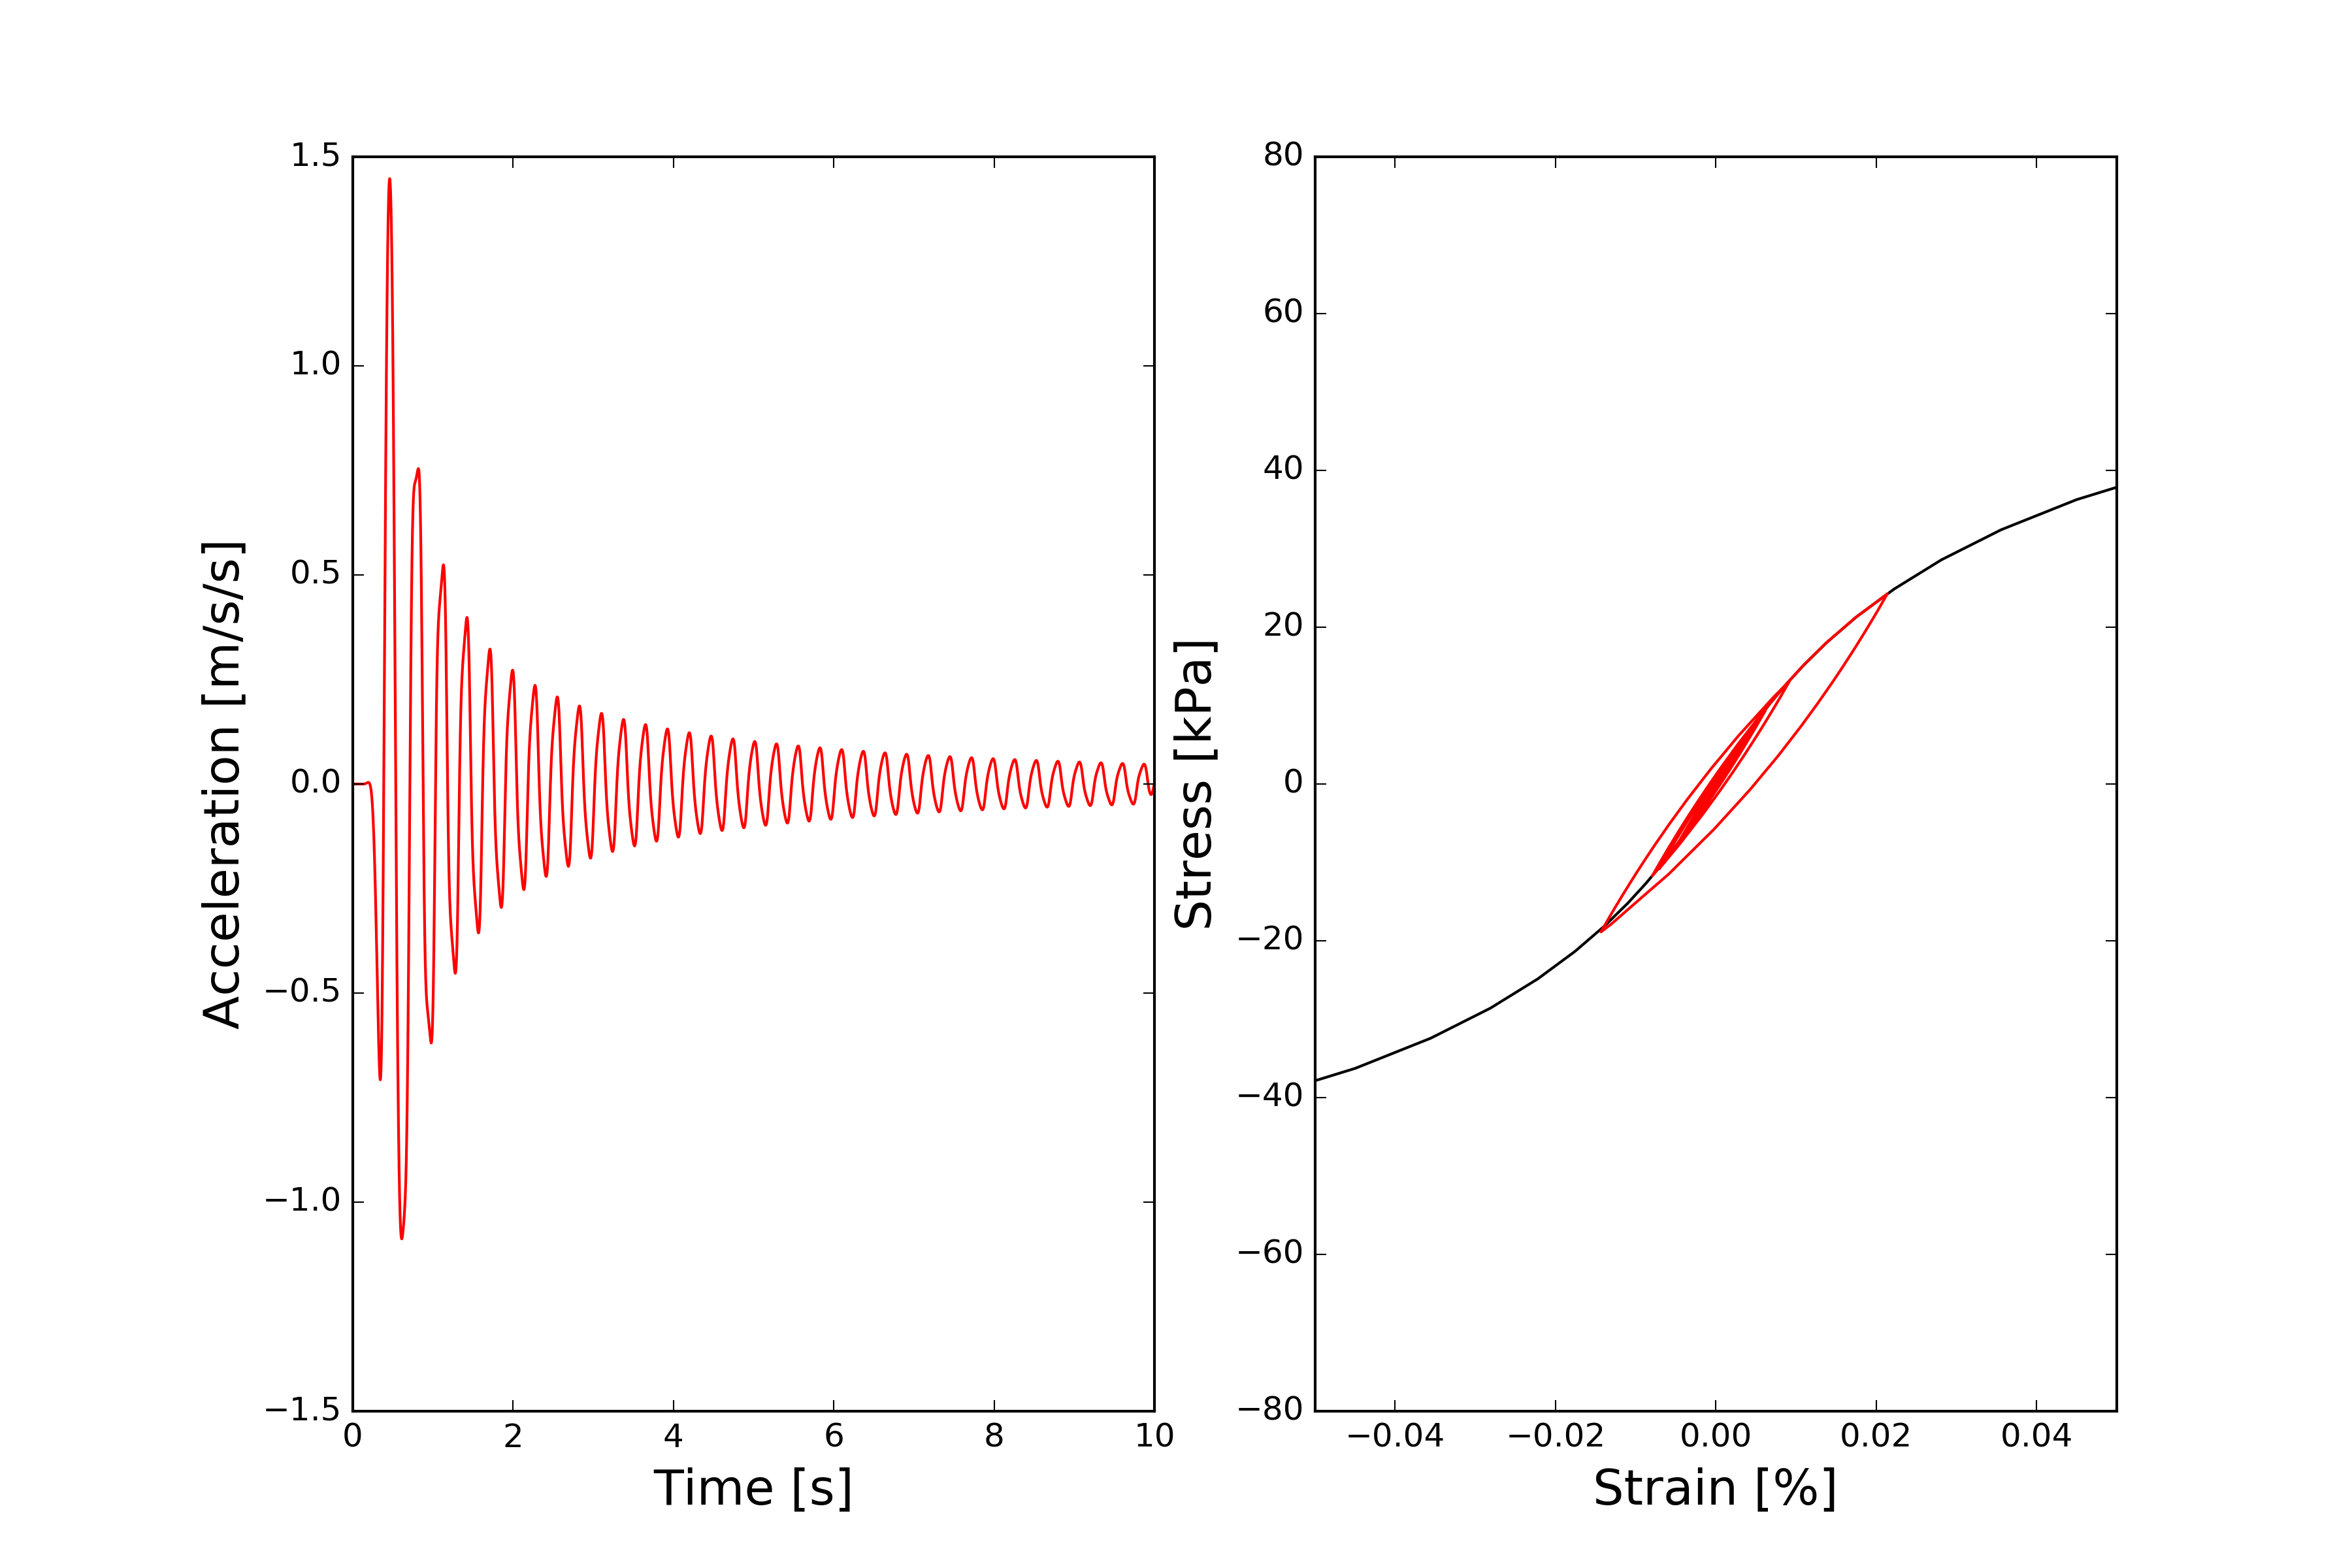
\includegraphics[scale=0.5]{figures/plot.eps} 
\captionof{figure}{Acceleration time histories at surface (left); Stress-strain curve at mid-column of P1 model (right).}
\label{plot} 
\vspace{1cm}
\end{center}



For plotting Fast Fourier transforms of a given file (acceleration or velocity time histories), fft.py file could be used. Resultant figure for WRLA model effective stress analysis is displayed in Figure \ref{fft}. \\


%% FIGURE : fft.png
\begin{center}
\leavevmode
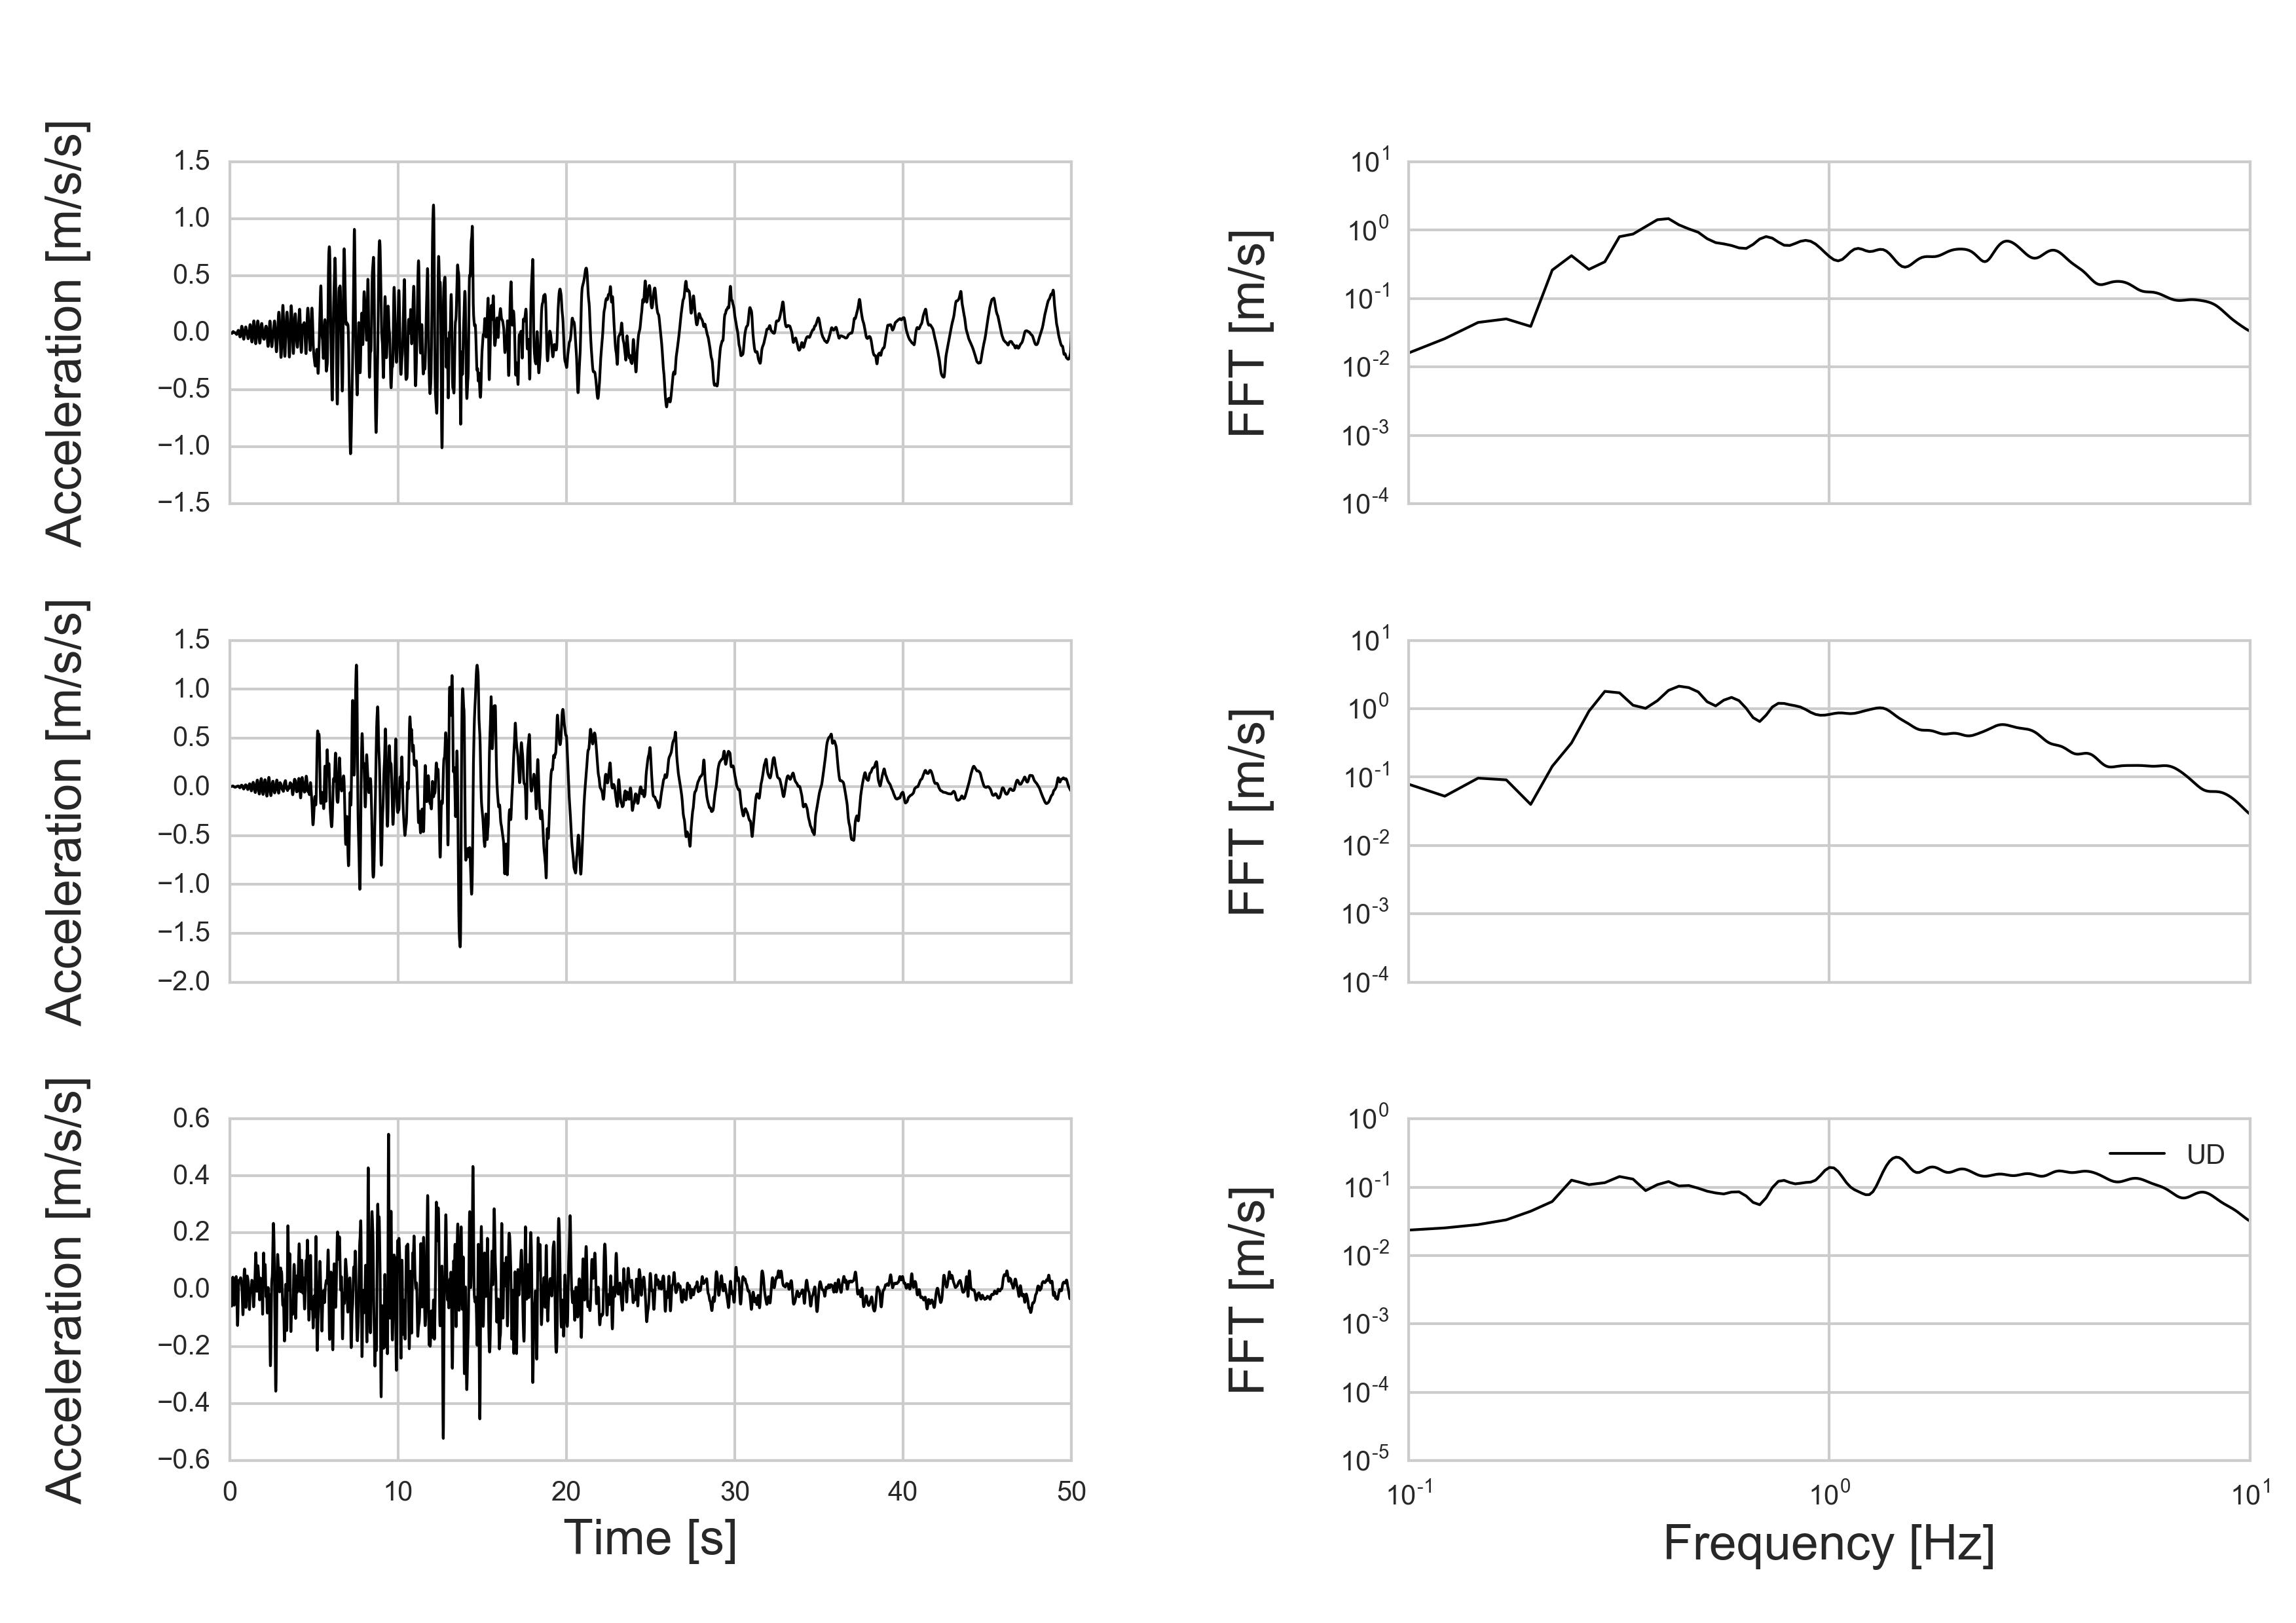
\includegraphics[scale=0.5]{figures/WRLA_acceleration_fft.eps} 
\captionof{figure}{Acceleration time histories at surface (left); Fast Fourier transform (right) for three directions of WRLA model effective stress analysis.}
\label{fft} 
\vspace{1cm}
\end{center}


For effective stress analyses, in order to visualize the changes in pore pressure excess, deviatoric plan, shear modulus and stress-strain curves, ‘effective\textunderscore changes.py’ file is ready to use. An example for WRLA model is shown in Figure \ref{eff}. \\


%% FIGURE : effective
\begin{center}
\leavevmode
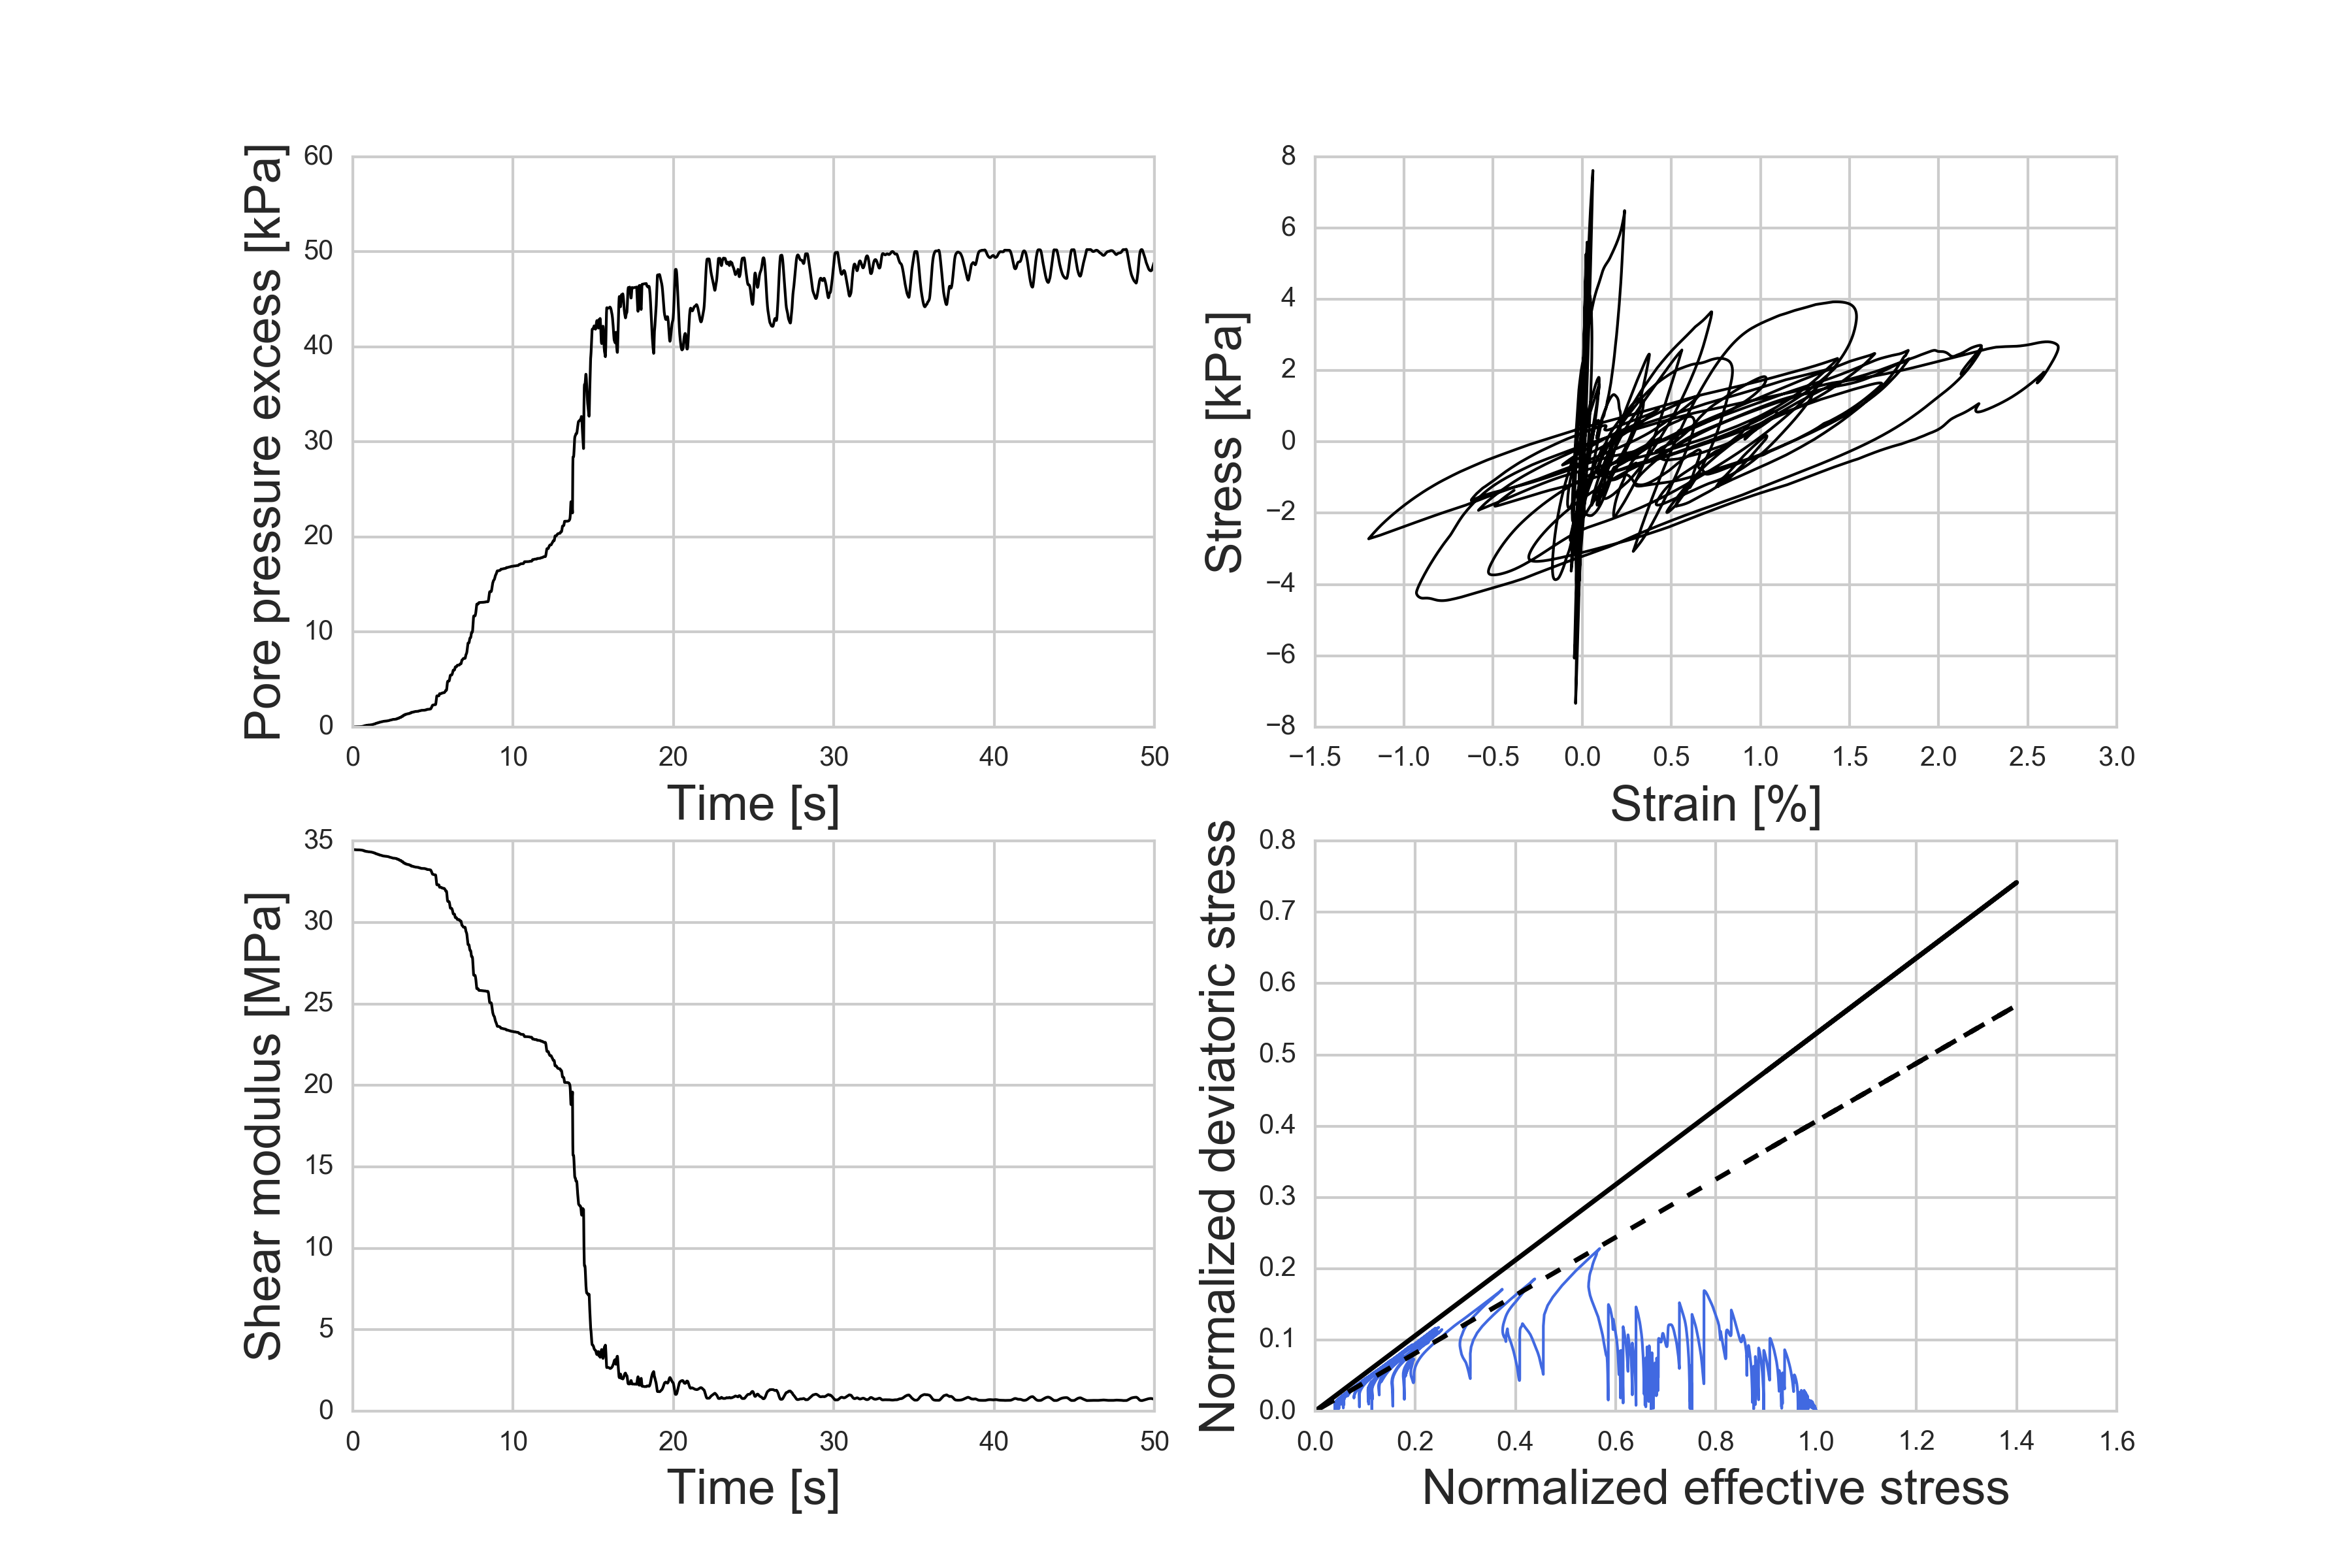
\includegraphics[scale=0.5]{figures/effective_stress_analysis.eps} 
\captionof{figure}{Pore pressure excess temporal change (left top); Stress-strain curve for EW-UD direction (top right); Change in shear modulus (bottom left); Deviatoric plan (bottom right) at GL-4 m for WRLA model effective stress analysis.}
\label{eff} 
\vspace{1cm}
\end{center}







\bibliographystyle{apalike}
\bibliography {Biblio}

\end{document}
